%%
%% Author: ncw135
%% 13/05/2019
%%

% Preamble
\documentclass[11pt]{article}

% Packages
\usepackage{amsmath}
\usepackage{graphicx}
\usepackage[a4paper]{geometry}
\usepackage{cleveref}
\usepackage{subcaption}

\title{Task1: Model building and simulation}

% Document
\begin{document}
    \maketitle

    In model1 (\cref{fig:model1:network}) A is produced from outside the system by constant, 0 order mass action kinetics. A is at steady state because
    A also undergoes degradation. Without stimulation by S, all that happens is that A finds a steady state. In
    the presence of S, A is reversibly converted to B. B stimulates the production of C which both undergoes
    spontaneous first order degradation and induces the degradation of B, thereby completing a negative feedback.

    \begin{figure}[h]

    \end{figure}


    \begin{figure}[h]
        \begin{subfigure}{0.7\textwidth}
            \centering
            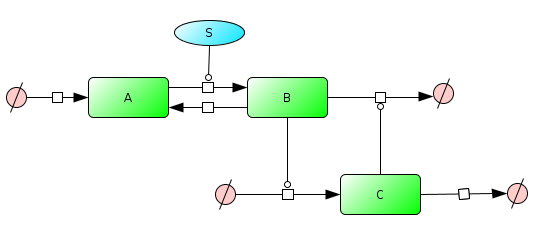
\includegraphics[width=\textwidth]{./figures/model1}
            \caption{Topology diagram of model 1.}
            \label{fig:model1:network}
        \end{subfigure}\\
        \centering
        \begin{subfigure}{0.45\textwidth}
            \centering
            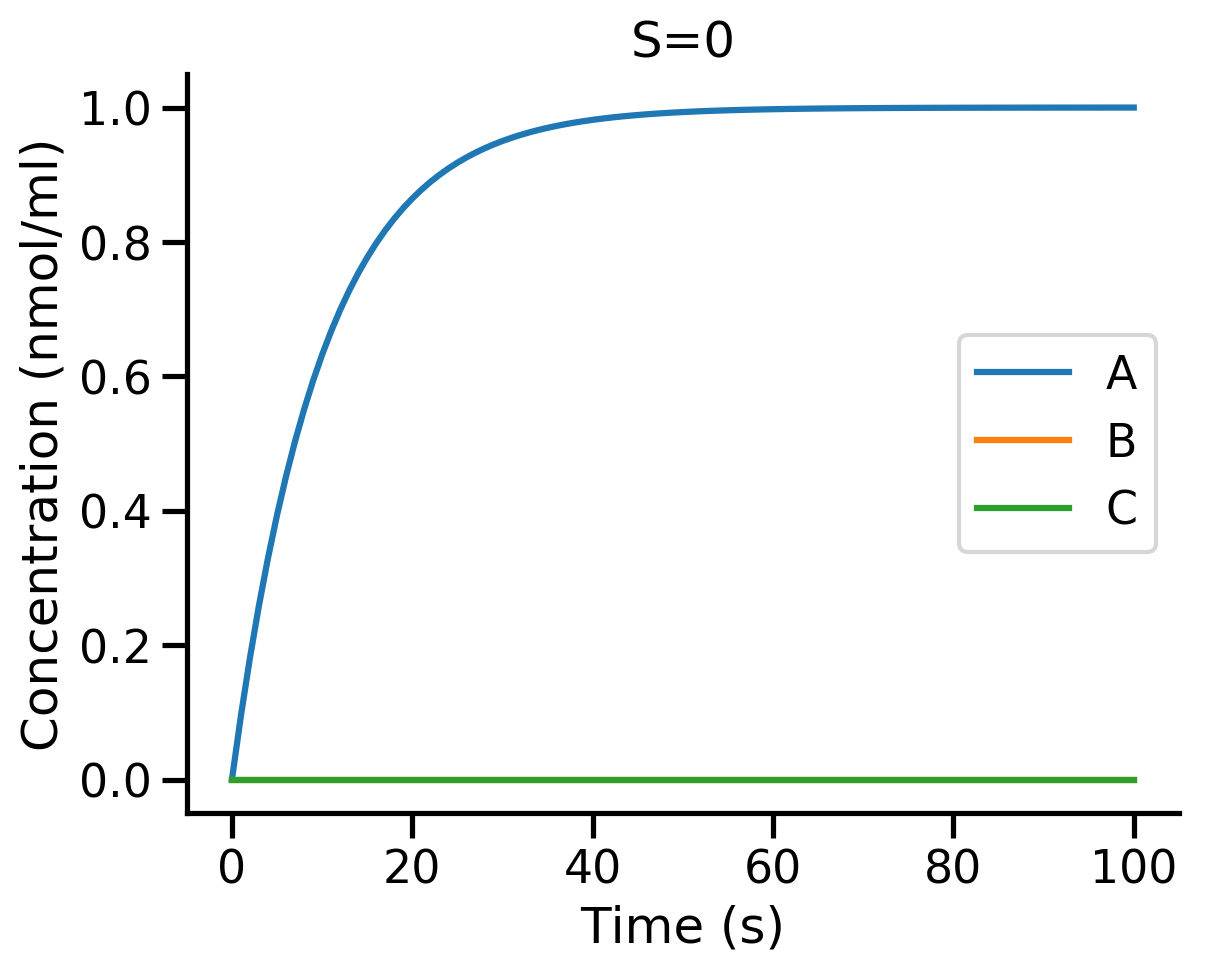
\includegraphics[width=0.9\textwidth]{./figures/WithoutS.png}
            \caption{}
            \label{a}
        \end{subfigure}
        \begin{subfigure}{0.45\textwidth}
            \centering
            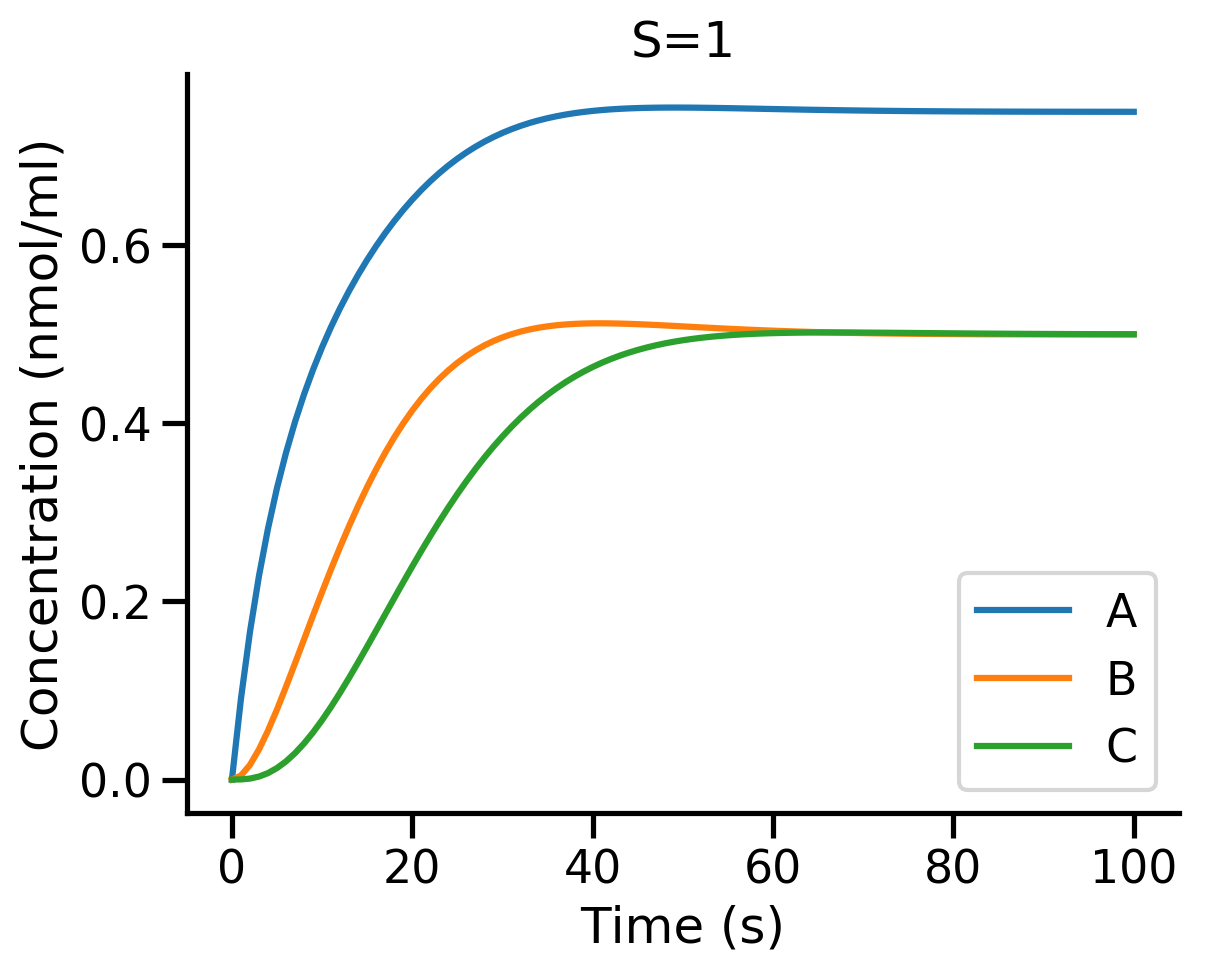
\includegraphics[width=0.9\textwidth]{./figures/WithS.png}
            \caption{}
            \label{b}
        \end{subfigure}
        \caption{Simulation of (a) model 1 with (b) $S_{0}=0$ and (c) $S_0=1$. Initial concentrations: $A=B=C=0$ and
        all kinetic parameters $k_1, ..., k_7 = 0.1$}
        \label{fig:model1}
    \end{figure}

    \begin{enumerate}
        \item Write the model equations with pen and paper
        \item Reproduce the simulation output in \cref{fig:model1} using Copasi
        \item Reproduce the simulation output using tellurium and antimony
        \item Change the rate law for the reaction where A gets converted to B by S to michaelis-menten kinetics using both Copasi and Antimony
        \item Change the rate law for the reaction where B is degraded by C to competitive inhibition kinetics using both Copasi and Antimony
    \end{enumerate}

    %    \subsection{}





\end{document}